\label{sec:evaluation}

We perform our evaluation on a quiescent 8-core system (dual
processor with 4 cores), and 8GB of RAM. Each processor is a 4-core
64-bit Intel Xeon running at 2.33 Ghz with a 4MB L2 cache. For
compatibility reasons, we compiled all applications to a 32-bit
target. All performance data is the average of 10 runs, excluding the
maximum and minimum values. Our evaluation answers the following questions:

\begin{itemize}
\item How effective is \sheriffdetect{} at finding and guiding programmers to resolve false sharing? (\textsection~\ref{sec:detective:effectiveness})
\item What is \sheriffdetect{}'s performance overhead? (\textsection~\ref{sec:results-detective-overhead})
\item How effectively does \sheriffprotect{} mitigate false sharing? (\textsection~\ref{sec:results-patrol-overhead})
\end{itemize}

\subsection{\sheriffdetect{} Effectiveness}
\label{sec:detective:effectiveness}

%Also, we are trying to verify whether \sheriff{} has false positives (mistakely report non-false sharing problems)
%and whether \sheriff{} has a lot of false negatives (miss some false sharing problems). 

We first evaluate \sheriffdetect{} with microbenchmarks we developed that exemplify a range of sharing scenarios. For comparison, we also present the
corresponding results of Intel's Performance Tuning Utility (PTU),
version 3.2~\cite{detect:ptu}.

\begin{comment}
\begin{figure}[!t]
\begin{lstlisting}
int count1 = 0; int count2 = 0;
void * thread1(void * param) {
  for(i = 0; i < COUNT_NUM; i++)
    count1++;		
}
void * thread2(void * param) {
  for(i = 0; i < COUNT_NUM; i++)
    count2++;       
}
\end{lstlisting}
\caption{Benchmark 1 (false sharing)   
\label{fig:benchmark1}}
\end{figure}

\begin{figure}[!t]
\begin{lstlisting}
int count[CORE_NUM];
void * thread(void * param) {
  int tid = (int)param;
  for(i = 0; i < COUNT_NUM; i++)
    count[tid]++;       
}
\end{lstlisting}
\caption{Benchmark 2 (pseudo sharing)
\label{fig:benchmark2}}
\end{figure}

\begin{figure}[!t]
\begin{lstlisting}
int count = 0; 
void * thread(void * param) {
  for(i = 0; i < COUNT_NUM; i++) 
    count++;       
}
\end{lstlisting}
\caption{Benchmark 3 (true sharing)
\label{fig:benchmark3}}
\end{figure}

\begin{figure}[!t]
\begin{lstlisting}
int count1 = 0; int count2 = 0;
void * thread1(void * param) {
  for(i = 0; i < COUNT_NUM; i++)
    count1++;       
}
void * thread2(void * param) {
  for(i = 0; i < COUNT_NUM; i++)
    count2++;       
}
int main() {
	spawn(&tid[0], thread1); join(tid[0]);
	spawn(&tid[1], thread2); join(tid[1]);
}
\end{lstlisting}
\caption{Benchmark 4 (noninterleaving-false sharing).
\label{fig:benchmark4}}
\end{figure}

\begin{figure}[!t]
\begin{lstlisting}
int * pcount1; int * pcount2;
void * thread1(void * param) {
  for(i = 0; i < COUNT_NUM; i++)
    pcount1[0]++;       
}
void * thread2(void * param) {
  for(i = 0; i < COUNT_NUM; i++)
    pcount2[1]++;       
}
int main() {
    pcount1 = malloc(16);
    spawn(&tid[0], thread1);  join(tid[0]); 
    free(pcount1);
    // New allocation here.
    pcount2 = malloc(16);
    spawn(&tid[1], thread2); join(tid[1]);
}
\end{lstlisting}
\caption{Benchmark 5 (heap-induced false positive).
\label{fig:benchmark5}}
\end{figure}
\end{comment}

Table~\ref{table:microbenchmarks} presents the results of this
evaluation. We can see that \sheriffdetect{} reports both false sharing
 and pseudo-sharing
 problems successfully, and correctly
ignores the benchmarks with no actual false sharing performance
impact (3--5). However, PTU reports false sharing for benchmarks 4 and
5. Note that benchmark 5 
triggers a false positive due to heap object reuse:
the two different allocations happen to occupy the same address.
\sheriffdetect{} avoids this false positive by cleaning up invalid counting
information.

%%%%%%%%%%%
%%% Whether we should add the pseudo code here.
%%%%%%%%%%%%

% \label{effect-application}

We next evaluate \sheriffdetect{}'s effectiveness at detecting false
sharing problems across a range of applications: the
Phoenix~\cite{phoenix-hpca} and PARSEC~\cite{parsec} benchmark suites,
and two open source multithreaded applications, \texttt{pbzip2} (a
parallel compressor) and \texttt{pfscan} (a parallel file scanner). We
use the simlarge inputs for all applications of PARSEC.  For Phoenix,
we chose parameters that allow the programs to run as long as
possible.~\footnote{As of this writing, we are unable to successfully
compile \texttt{raytrace} and \texttt{vips}, and \sheriff{} is
currently unable to run \texttt{x264}, \texttt{bodytrack},
and \texttt{facesim}. \texttt{Freqmine} is not included because it
does not support \pthreads{}. }
 
%%%%%%%%%%%%%%%%%%%%%%%%%%%%%%%%%%%%%%%%%%%%%%%%%%%%%%%%%%%%%%%%%%%%%%%%%%%%%%%%%%%%%%%%%%%%%%
%%%%%% Use a table to listed some data about benchmarks and description of these benchmarks.
%%%%%% List how many false sharing objects are reported, how many objects are false sharing problems. 
%%%%%% How many commits inside, how many pages are written totally, how many allocations are invoked. 
%%%%%% Footprint of those protected pages, shared pages. 
%%%%%%%%%%%%%%%%%%%%%%%%%%%%%%%%%%%%%%%%%%%%%%%%%%%%%%%%%%%%%%%%%%%%%%%%%%%%%%%%%%%%%%%%%%%%%%



\begin{table}[!t]
\centering
\begin{tabular}{l|r|r}
\hline
{\bf \small Benchmark} & {\bf \small PTU} & {\bf \small \sheriffdetect{}} \\
 & {\em cache lines} & {\em objects}\\
\hline
\small \texttt{blackscholes} & 0 & 0 \\
\small \texttt{canneal} & 1 & 1 \\
\small \texttt{dedup} & 0 & 0 \\
\small \texttt{ferret} & 0 & 0\\
\small \texttt{fluidanimate} & 3 & 1 \\
\small \texttt{histogram} & 0 & 0 \\
\small \texttt{kmeans} & 1,916 & 2 \\
\small \texttt{linear\_regression} & 5 & 1 \\
\small \texttt{matrix\_multiply} & 468 & 0\\
\small \texttt{pbzip2} & 14 & 0 \\
\small \texttt{pca} & 45 & 0 \\
\small \texttt{pfscan} & 3 & 0 \\
\small \texttt{reverse\_index} & \textbf{N/A} & 5 \\
\small \texttt{streamcluster} & 9 & 1\\
\small \texttt{string\_match} & 0 & 0 \\
\small \texttt{word\_count} & 4 & 3\\
\small \texttt{swaptions} & 196 & 0\\
\hline
\small \textbf{\em Total} & 2,664 & 14 \\
\hline
\end{tabular}
\caption{Detection results for PTU and \sheriffdetect{}. For PTU, we show 
how many cache lines are reported as (potentially) falsely shared. For \sheriffdetect{},
we provide the number of objects reported (with significance filtering turned off).
``N/A'' indicates that PTU failed because it ran out of memory.
\label{table:detection}}
\end{table}

Table~\ref{table:detection} shows that \sheriffdetect{} reveals false
sharing in seven out of seventeen benchmarks (when filtering for low
performance impact is disabled; see below). \sheriffdetect{} detects
false sharing
in four benchmarks from the Phoenix suite and
three from the PARSEC suite.
However, for three of these benchmarks
(\texttt{kmeans}, \texttt{canneal}, and \texttt{fluidanimate}), the
average number of interleavings per cache line is lower than 10, indicating
that the false sharing would not have a significant performance
impact;
\sheriffdetect{} is normally configured not to report these.

%\sheriffdetect{} ... The false sharing detected includes both inter-object and intra-object false sharing. 


\begin{figure}[!t]
\begin{lstlisting}
int * use_len;
void insert_sorted(int curr_thread) {
   ......	
   // After finding a new link
   (use_len[curr_thread])++;
   ......	
}
\end{lstlisting}
\caption{False sharing detected by \sheriffdetect{} in \texttt{reverse\_index}. False sharing arises when adjacent threads 
modify the \texttt{use\_len} array. 
\label{fig:reverseindex}}
\end{figure}

In \texttt{reverse\_index} and \texttt{word\_count}, multiple threads
repeatedly modify the same heap object. A simplified version of the
code is shown in Figure~\ref{fig:reverseindex}. Using a
thread-local copy avoids false sharing: each thread can operate on a
temporary variable and modify the global \texttt{use\_len} only at the
end of the thread.

\texttt{Linear\_regression}'s false sharing problem is slightly different 
(see Figure~\ref{fig:linear_regression}). 
In this case, two different threads falsely share the same cache line if the
structure \texttt{lreg\_args} is not cache line aligned. This problem
can easily be avoided simply by padding the structure \texttt{lreg\_args}.


\begin{figure}[!t]
\begin{lstlisting}
struct {
  long long SX;
  long long SY;
  long long SXX;
  ......
} lreg_args;

void *lreg_thread(void *args_in) {
  struct lreg_args * args = args_in;
  for(i = 0; i < args->num_elems; i++) {
    args->SX  += args->points[i].x;
    args->SXX += args->points[i].x 
   	         * args->points[i].x;
  }
  ......	
}
\end{lstlisting}
\caption{False sharing detected by \sheriffdetect{} in \texttt{linear\_regression}.
Each thread is passed in a pointer to a struct as an argument, but the struct is smaller than a
cache line (52 bytes), so two different threads write to the same cache line simultaneously. 
\label{fig:linear_regression}}
\end{figure}

The false sharing detected in \texttt{streamcluster} (one of
the PARSEC benchmarks) is similar to the false sharing 
in \texttt{linear\_regression}. 

% CC: This seems obvious, so I left it out
% two different threads write to the same cache line.  

Examination of the source code indicates that the author tried to avoid false sharing 
by padding, but the amount of padding, 32 bytes, was insufficient
to accomodate the actual physical cache line size 
used in the evaluation (64 bytes).  Setting
the \texttt{CACHE\_LINE} macro to 64 bytes eliminates the
false sharing.

The performance of these four benchmarks is listed in
Table~\ref{table:perfafterfix}, before and after fixing the false
sharing issues that \sheriffdetect{} identifies.  To understand 
the differences in performance improvements, we modified the code
to compute the number of updates to these falsely shared objects.
Updates listed here are the \emph{maximum} possible number of interleaving
writes of these objects; the actual number of interleaving writes
depends on scheduling.

The \texttt{reverse\_index} and \texttt{word\_count} benchmarks do not
exhibit substantial performance improvements after removing false
sharing because the number of updates is relatively low. For example,
the maximum number of interleaved updates for \texttt{reverse\_index}
is 416,000. The \texttt{streamcluster} benchmark has around 28 million
updates, and eliminating false sharing provides a modest performance
improvement (5.4\%). The most dramatic improvement is
for \texttt{linear\_regression}. After removing its false sharing, it
runs $9\times$ faster.

% Note that despite its
%relatively low numbers of updates, as the
%number of threads grow, the false sharing
%in \texttt{reverse\_index} will eventually become a performance bottleneck.

\begin{figure*}[!t]
\centering
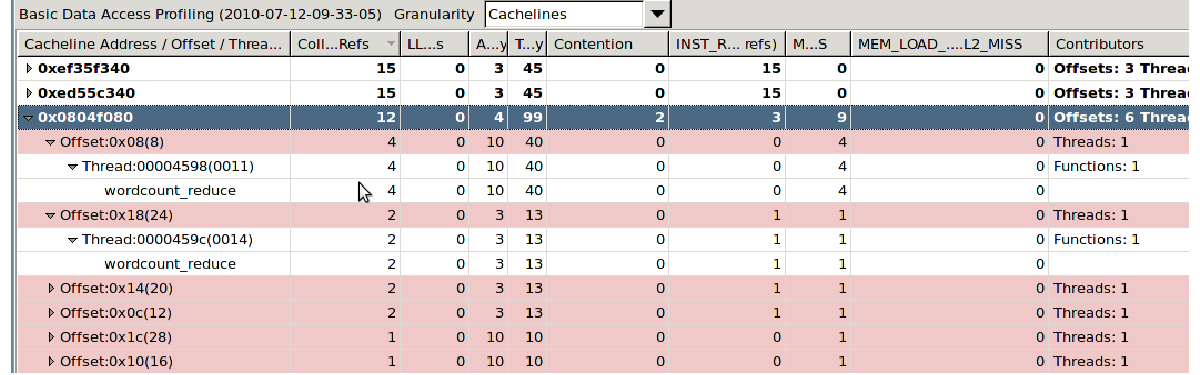
\includegraphics[width=6in]{figure/wordcount}
\caption{A fragment of Intel Performance Tuning Utility's report for \texttt{word\_count} (see Section~\ref{evaluation:comparison}); the full report is 863 lines long.
\label{fig:wordcount}}
\end{figure*}

\subsubsection{\sheriffdetect{} vs. PTU}
\label{evaluation:comparison}

%%%%%%%%%%%%%%%%%%%%%%%%%%%%%%%%%%%%%%%%%%%%%%%%%%%%%%%%%%%%%%
%%%%% OUTPUT here %%%%%%%%%%%%%%%%%%%%%%%%%%%%%%%%%%%%%%%%%%%%
%%%%%%%%%%%%%%%%%%%%%%%%%%%%%%%%%%%%%%%%%%%%%%%%%%%%%%%%%%%%%%%

To evaluate \sheriffdetect{}'s effectiveness at finding false
sharing, we compare it to Intel's Performance Tuning
Utility (PTU), a commercial product which represents
the state of the art for detecting false sharing.

This comparison evaluates the number of reports that each tool
generates, and the effectiveness of each at helping the programmer
find and resolve actual instances of false sharing.

\paragraph{Reporting.}
For PTU, we list the number of cache lines reported as possibly
falsely-shared. To locate a single case of false sharing, a programmer
must sift through every one of these reports. \sheriffdetect{}
reports sharing at the object granularity.

%normally only reports sharing in terms of objects rather than cache
%lines, but the table lists both objects and the number of cache lines
%to facilitate comparison with PTU.

\begin{table}
\centering
\begin{tabular}{l|r|r|r|r}
\hline
{\bf \small Benchmark} & {\bf \small Orig} & {\bf \small Mod} & {\bf \small Speedup} & {\bf \small Updates}\\
& (s) & (s) & & (M)\\
\hline
\small \texttt{linear\_regression} & 3.40 & 0.37 & 818\% & 1323.6\\
\small \texttt{reverse\_index} & 2.08 & 2.03  & 2.4\% & 0.4\\
\small \texttt{streamcluster} & 2.78 & 2.63 & 5.4\% & 28.7\\
\small \texttt{word\_count} & 2.20 & 2.18 & 1\% & 0.3\\
\hline
\end{tabular}
\caption{Performance data for benchmarks with significant false sharing, as reported by \sheriffdetect{}. 
``Orig'' and ``Mod'' are the runtimes before and after fixing the false sharing
revealed by \sheriffdetect{}.
All data are obtained running with \pthreads{}.
``Updates'' is the maximum number of updates to falsely-shared cache lines.
\label{table:perfafterfix}}
\end{table}

From the results listed in Table~\ref{table:detection}, we can see
that \sheriffdetect{} imposes a far lower burden on the
programmer. Across all of the benchmarks, PTU indicates the need to
examine 2,664 cache lines overall (not
including \texttt{reverse\_index}, which PTU cannot run). By
contrast, \sheriffdetect{} reports just 14 objects as potential source
of false sharing.  After increasing its significance threshold
parameter,
\sheriffdetect{} reports just 4 objects, all of which are truly
false sharing.

%The column "False-negatives" shows possible false negatives of \sheriffdetect{} which we got results 

Several factors lead to this difference.  
%TONGPING_BEGIN
First, \sheriffdetect{} reports objects rather than cache lines, which reduces 
the number of reports when one callsite is the source of a number of
allocations (as in \texttt{kmeans}) 
or when one object spans multiple cache lines (as in \texttt{reverse\_index}).
Second, \sheriffdetect{} distinguishes true from false sharing, reducing the number of reported
items.  Finally, \sheriffdetect{} only reports those objects with
interleaving writes above a threshold, which
significantly reduces the number of reports. 

%  Third, \sheriffdetect{} reports
% corresponding objects instead of cache lines, which also reduces the
% number of reports if one object spans multiple cache lines.
%TONGPONG_END

%Readers wonder whether \sheriffdetect{} misses some critical false sharing problems? 

\paragraph{Ease of locating false sharing.}
To illustrate how \sheriffdetect{} can precisely locate false sharing instances, we 
use the \texttt{word\_count} benchmark as
a representative example. Our experience with diagnosing other false sharing issues is similar. Below is an extract of \sheriffdetect{}'s report for \texttt{word\_count}:

\begin{verbatim} 
1st object, cache interleaving writes 
13767 times (start at 0xd5c8e140). 
Object start 0xd5c8e160, length 32. 
It is a heap object with callsite:
[0] ./wordcount_pthreads.c:136
[1] ./wordcount_pthreads.c:441
\end{verbatim}

\noindent
Line 136 (\texttt{wordcount\_pthreads.c}), 
contains the following memory allocation:

\begin{verbatim}
use_len=malloc(num_procs*sizeof(int));
\end{verbatim}

\noindent
Grepping for \texttt{use\_len}, a global pointer, quickly leads to this line:

\begin{verbatim}
use_len[thread_num]++;
\end{verbatim}

Now it is clear that different threads are modifying the same object
(\texttt{use\_len}). Fixing the problem with 
thread-local copies of this object is now straightforward~\cite{detect:intel}.

By contrast, compare PTU's output for the same benchmark, shown in
Figure~\ref{fig:wordcount}.  Finding this problem is far more
complicated with PTU. The full report consists of 863 lines
describing cache lines and the functions that access them, not
individual objects. The task of finding false sharing is further
exacerbated by the fact that many of these reports are false
positives. PTU is also unable to effectively rank the performance
impact of false sharing instances. The ``Collected Data Refs'' metric
(the second column) is inaccurate at best: for this example, PTU only
reports 12 references, while \sheriffdetect{} observes 13,767
references.

%That is why we cannot relying on PTU to do the analysis of false sharing
%problems given the large number of cache lines involved. 

\subsection{ \sheriffdetect{} Performance}
\label{sec:results-detective-overhead}

\begin{figure*}[!t]
\centering
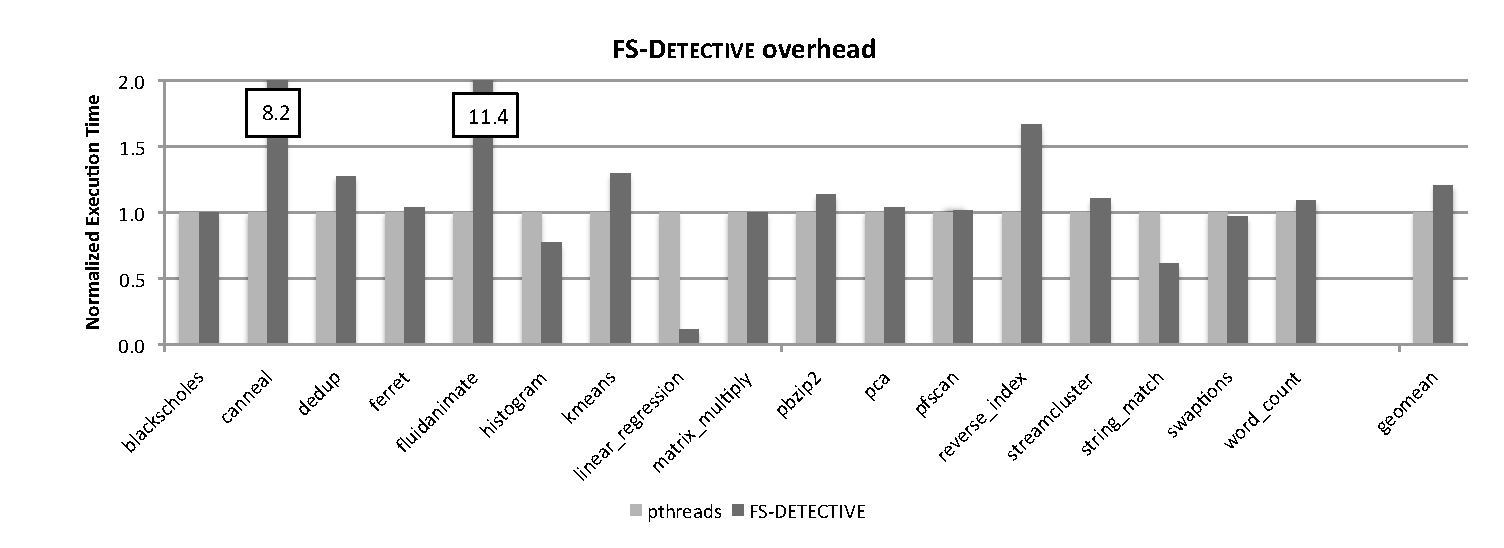
\includegraphics[width=6in]{figure/detectiveperf}
\caption{\sheriffdetect{} overhead across two suites of benchmarks,
  normalized to the performance of the \pthreads{} library (lower is better). 
  With two exceptions, its overhead is quite low (on average, just $20\%$).
\label{fig:overhead}}
\end{figure*}


Figure~\ref{fig:overhead} presents the runtime overhead of \sheriffdetect{} versus
\pthreads{} across our benchmark suites. \sheriffdetect{} executes with surprisingly
low overhead: $20\%$ on average, with the exception of three outliers.

There are two benchmarks on which \sheriffdetect{} does not perform
particularly well. One is \texttt{canneal}, where the performance overhead of \sheriffdetect{}
is about $8\times$ compared to \pthreads{}, while \texttt{fluidanimate}'s overhead is approximately
$11\times$ slower than that using \pthreads{}. 

% \texttt{canneal},
%the problem is that it dirties a large number of pages (2.9
%million). \texttt{fluidanimate} also dirties a large number of pages
%(2.1 million), but in addition, it has an unusually large number of
%transactions (18.7 million).


\begin{comment}
\begin{table}
\centering
\begin{tabular}{|l|r|r|r|}
\hline
{\bf \small Benchmark} & {\bf \small Trans} & {\bf \small DirtyPages} & {\bf \small Runtime} \\
 & {\#} & {\#} & {s}\\
\hline
\small \texttt{blackscholes} & 24 & 986 & 10.36 \\
\small \texttt{canneal} & 1,064 & 3,485,220 & 86.72 \\
\small \texttt{dedup} & 45,563 & 62,515 & 1.74 \\
\small \texttt{ferret} & 1,052,027 & 149,188 & 6.5\\
\small \texttt{fluidanimate} & 16,718,127 & 3,297,999 & 17.64 \\
\small \texttt{histogram} & 23 & 29 & 0.33 \\
\small \texttt{kmeans} & 3,936 & 7,204 & 11.56 \\
\small \texttt{linear\_regression} & 24 & 17 & 0.38 \\
\small \texttt{matrix\_multiply} & 24 & 3,939 & 19.02 \\
\small \texttt{pbzip2} & 1,015,388 & 34,597 & 2.04 \\
\small \texttt{pca} & 46 & 11,667 & 21.37\\
\small \texttt{pfscan} & 131 & 98 & 0.37  \\
\small \texttt{reverse\_index} & 60,714 & 130,061 & 3.46\\
\small \texttt{streamcluster} & 127,318 & 107,968 & 3.07\\
\small \texttt{string\_match} & 24 & 26 & 2.08\\
\small \texttt{swaptions} & 24 & 852 & 4.09\\
\small \texttt{word\_count} & 88 & 8,575 & 2.4\\
\hline
\end{tabular}
\caption{Characteristics of benchmarks in \sheriffdetect{}. The number of ``transactions'' (epochs between synchronization points) and the number of dirtied pages are the primary sources of overhead.
\label{table:characteristics}}
\end{table}
\end{comment}


\begin{figure*}[!t]
\centering
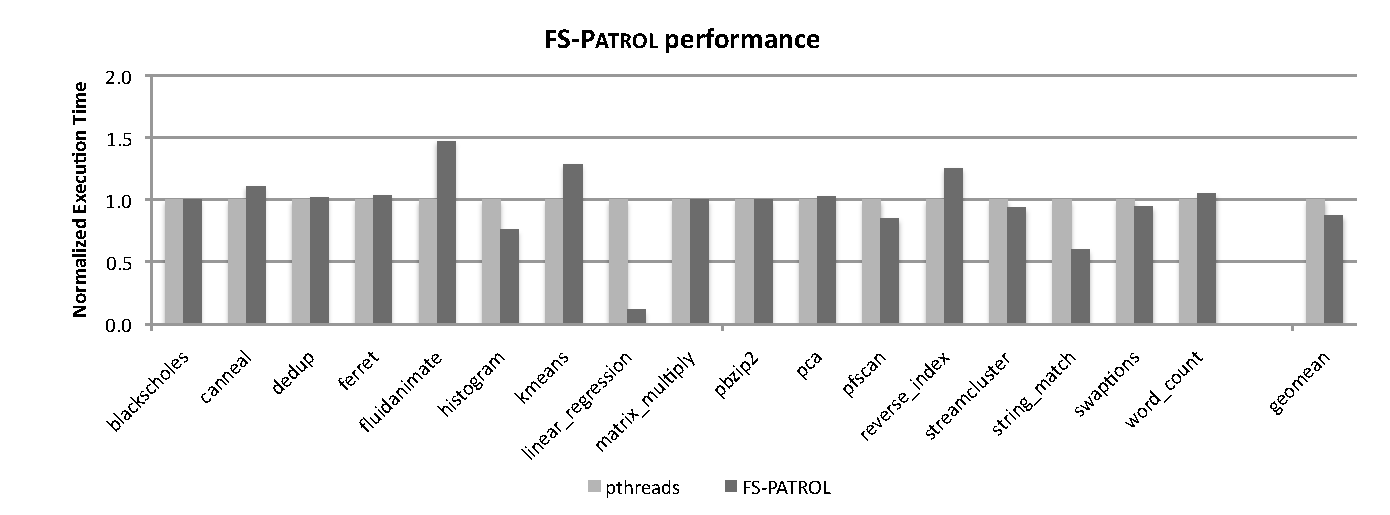
\includegraphics[width=6in]{figure/patrolperf}
\caption{\sheriffprotect{} performance,
  normalized to the performance of the \pthreads{} library (see
  Section~\ref{sec:results-patrol-overhead}; lower is better). For applications with
  significant false sharing, \sheriffprotect{} can substantially increase performance.
\label{fig:patrol}}
\end{figure*}

\begin{table}[!t]
\centering
\begin{tabular}{l|r|r}
\hline
{\bf \small Benchmark} & \multicolumn{2}{c} {\bf \small Normalized Runtime} \\
% \cline{2-3}
 & {\bf \small \sheriffdetect{} }  & {\bf \small \sheriffprotect{}} \\
\hline
\small \texttt{blackscholes} & 1.00 & 1.00 \\
\small \texttt{canneal} &  8.23 & 1.11 \\
\small \texttt{dedup} & 1.27 & 1.02 \\
\small \texttt{ferret} & 1.03 & 1.03\\
\small \texttt{fluidanimate} & 11.39 & 1.47 \\
\small \texttt{histogram} & \textbf{0.77} & \textbf{0.76} \\
\small \texttt{kmeans} & 1.29 & 1.28 \\
\small \texttt{linear\_regression} & \textbf{0.12} & \textbf{0.11} \\
\small \texttt{matrix\_multiply} & 1.00 & 1.00 \\
\small \texttt{pbzip2} & 1.13 & 1.00 \\
\small \texttt{pca} & 1.04 & 1.03 \\
\small \texttt{pfscan} & 1.02 & \textbf{0.85} \\
\small \texttt{reverse\_index} & 1.67 & 1.25 \\
\small \texttt{streamcluster} & 1.10 &  \textbf{0.94} \\
\small \texttt{string\_match} & \textbf{0.61} & \textbf{0.60} \\
\small \texttt{swaptions} & \textbf{0.97} & \textbf{0.94} \\
\small \texttt{word\_count} & 1.09 & 1.05\\
\hline
\small \textbf{\em Geomean} & 1.21 & \textbf{0.87} \\
\hline
\end{tabular}
\caption{Detailed execution times with \sheriffdetect{} and \sheriffprotect{}, normalized to execution with the \pthreads{} library; numbers below 1 (boldfaced) indicate a speedup over \pthreads{}.
\label{table:detailedperf}}
\end{table}

The first reason for these overheads is that both benchmarks trigger a
high number of dirtied pages (3.4 million and 2.15 million,
respectively). For each dirty page, \sheriffdetect{} applies memory
protection twice, creates the copy-on-write version and twin page,
checks for false sharing at every checking period, and finally commits
updates to the shared mapping. Copying alone is a major part of the
overhead associated with dirty pages, since one dirty page needs at
least three copies.  For \texttt{canneal}, copying alone accounts for
about 20 seconds of additional execution time.

\texttt{fluidanimate} also runs slowly with \sheriffdetect{} because of an unusually
high number of transactions (16.7 million). Examination of the source
code of \texttt{fluidanimate} reveals frequent locking and unlocking.
\sheriff{} replaces lock calls with their interprocess variants and
triggers a transaction end and begin for each, adding overhead if
there are shared pages (as here).

While these outliers force \sheriffdetect{} to run
slowly, \sheriffdetect{}'s overhead is generally acceptable and far
lower than most previous tools.

\texttt{linear\_regression} is an outlier in the opposite direction: with \sheriffdetect{}, it runs
$8\times$ faster than with \pthreads{}. The reason is a serious false
sharing issue (see Table~\ref{table:perfafterfix}) that
both \sheriffdetect{} and
\sheriffprotect{} eliminate automatically, thus dramatically improving
performance. Other cases where \sheriffdetect{}
outperforms \pthreads{} are also due to false sharing
elimination; \sheriffprotect{} further reduces overhead for these and
other applications, as the next section describes.


%%%%%%%%%%%%%%%%%%%%%%%%%%%%%%%%%%%%%%%5
%%%% Some data to list the effectiveness of this tool.
%%%%%% How many caches are carried for each test case. 
%%%%%% Whether all caches has false sharing problem.
%%%%%%%%%%%%%%%%%%%%%%%%%%%%%%%%%%%%%%%
\subsection{Effectiveness of \sheriffprotect{}}
\label{sec:results-patrol-overhead}

Here, we examine the effectiveness of \sheriffprotect{} at mitigating
false sharing; Figure~\ref{fig:patrol} presents execution times
versus \pthreads{}. For most applications,
\sheriffprotect{} either has no effect on performance (when there is no false sharing to eliminate) or
improves it. Table~\ref{table:detailedperf} provides detailed
performance numbers for both \sheriffprotect{} and \sheriffdetect{}.

% munmap() call to unmap about 400M's file,
%we currently are not sure about why multi-process framework can
%perform better in this case.

For three applications, \sheriffprotect{} degrades performance by up
to 47\% versus \pthreads{}. For \texttt{kmeans}, which creates over 375
threads per second, the added cost stems from using processes instead
of threads. While process creation on Linux is relatively cheap, it is
still more expensive than creating threads.

The slowdowns for \texttt{reverse\_index} and \texttt{fluidanimate}
are due to more subtle technical details of the processes-as-threads
framework. \sheriff{} uses a file-based mapping to connect the private
and shared mappings. The Linux page fault handler does more work when
operating on file-based pages than on anonymous pages (the normal case
for heap-allocated pages). For example, the first write to a
file-mapped page repopulates information from the file's page table
entry. In addition, the shared store for all heap pages is initially
set to \texttt{MAP\_SHARED}, so writing to one shared page can cause a
copy-on-write operation in the kernel even when there is only one
user. As future work, we plan to investigate extending the kernel with an
additional mapping mode to eliminate this overhead.

\sheriffprotect{} improves the performance of the programs implicated
by \sheriffdetect{} as suffering from false sharing, as well as several
others. For example, \texttt{histogram} also runs substantially faster
with \sheriffprotect{} (24\%), although we currently are not certain
why this is the case.
\texttt{string\_match} runs 40\% faster because of false sharing
caused by the \pthreads{} heap allocator (which is why
\sheriffdetect{} does not find it). The most dramatic
improvement comes from
\texttt{linear\_regression}, which runs $9\times$ faster than with
\pthreads{} because \sheriffprotect{} eliminates its serious false
sharing (see Table~\ref{table:perfafterfix}).  These results
show that \sheriffprotect{} is effective at mitigating false sharing
without the need for programmer intervention or access to source code.
